\section{Conclusions}

We have developed a novel theoretical and computational framework to model
and simulate the fully non-linear dynamics of a compressible active nematic gel, both confined to a plane and on a deformable surface. More specifically,
\begin{enumerate}
	\item We have developed a general theoretical framework for active nematic gels based on Onsager's variational formalism, according to which the fully coupled and nonlinear dynamics minimize a functional where free-energy release, dissipation and power input compete. This method provides an unambiguous roadmap to derive complex governing equations from fundamental building blocks and their coupling. For instance, going from a 2D active nematic gel to one on a deformable surface only requires expressing the free-energy, the dissipation potential and the power input covariantly, and then applying the same variational procedure. We have particularized our general framework to active nematic gels which, contrary to common models for incompressible nematic liquid crystals, are not bound by topological nematic constraints since isotropic states can be favorable, and can develop strong density variations, which are essential to understand the active self-organization of the actin cytoskeleton. 
	\item We have developed a computational framework to solve the governing equations of an active nematic gel on 2D fixed domains with arbitrary boundary conditions, on two-dimensional domains with moving boundaries, on axisymmetric deformable  surfaces and on general deformable  surfaces. Onsager's variational formalism naturally lends itself to space and time discretization. For space discretization, we use linear, B-Spline or subdivision finite elements depending on the context. For time discretization, we resort to backward Euler schemes and to a time-incremental version of Onsager's variational method.
	\item We have applied this theoretical and computational framework to understand a variety of biological problems revolving around the active self-organization and dynamics of nematic structures.  In the first part of the thesis focusing on gels confined to a 2D plane, 
	\begin{enumerate}
	\item we have studied the self-assembly of a dense and nematic contractile ring at the edge of a hole or wound in an initially quiescent, isotropic and uniform gel, leading to spontaneous wound healing. 
	\item We have also studied the spontaneous formation and motion of nematic defects and active flows in dense colonies of elongated cells. 
	\item Finally, we have studied the active self-organization of patterns of dense nematic structures starting from quiescent, isotropic and uniform gels. We have mapped how model parameters control the architecture, geometry and dynamics of such patterns. Hence, this study establishes a framework to understand the polymorphism of the actin cytoskeleton. Importantly, this theory provides a mechanism for the self-organization of patterns of dense nematic bundles as observed in a variety of cellular contexts, Figs.~\ref{chap_1_fig_1} and \ref{chap_1_fig_22}. This mechanism imposes requirements on the relation between nematic order and activity in the theory, which we substantiate using out-of-equilibrium discrete network simulations.
	\end{enumerate}
	In the second part of the thesis focusing on active nematic gels on deformable surfaces
	\begin{enumerate}
	\item we have reproduced the self-organization of a dense and nematic cytokinetic ring from either an equatorial over-activity or as a symmetry-breaking spontaneous mode. We have shown that the nematic coupling facilitates complete cell division and accelerates the process. We have also briefly explored the competition between cytokinetic and polarized symmetry-breaking dynamical modes. 
	\item Turning to an inextensible, active and nematic liquid crystal confined to a vesicle, we have examined the interplay between nematic defects and curvature.
	\end{enumerate}
\end{enumerate}

\section{Future work}

This thesis is also a foundation to develop the following research avenues, which are either proposed or actual ongoing research projects.

\subsection*{Dynamics of topological defects in nematic cell monolayers}

  Spindle-shaped cells such as fibroblasts, myoblasts, or some epithelial cells self-organize into domains with high nematic order and $\pm 1/2$ topological defects  \cite{duclos2017, guillamat2020}. These multicellular defects organize well-defined orientational patterns that lead to reproducible flow and force fields generated by active processes in the actomyosin cytoskeleton. Although the interplay between orientational patterns around topological defects and forces has been elucidated for epithelial cell monolayers \cite{balasubramaniam2021}, it remains elusive for mesenchymal tissues, where, mainly due to a lower cell-cell adhesion and apolar cell migration, defect dynamics are notably different. %In particular, we are interested in understanding the mechanical roles of topological defects in these systems.
To understand the mechanisms underlying nematic, flow, and force patterns around possibly motile defects in mesenchymal-like cell monolayers, we plan to combine quantitative observations of in vitro cell cultures and numerical simulations based on an active nematic gel theory. We plan to compare experimentally measured nematic orientation fields, flow fields and monolayer-substrate traction fields around $\pm 1/2$ topological defects along with defect dynamics with theoretical prediction to establish the interplay between active and passive forces in the system. Once the active nematic gel parameters have been identified, we plan to use the model to devise strategies to rationally manipulate cellular active matter around nematic defects.
%This project aims to characterize the mechanisms underlying defect motility in mesenchymal-like cell monolayers by using a combination of in vitro cell culture experiments and numerical simulations. The latter are based on the conception that the defect dynamics result from an interplay between elastic nematic energy, active processes, and dissipative effects, namely viscous flow of cells and friction from the interaction between the cells and the substrate.
%In our experimental setup,  we prepare nematic monolayers of fibroblasts on soft, cell-deformable, elastomeric substrates ($\sim$kPa) coated with nanometric fluorescent tracer beads. We then simultaneously obtain images of the cell monolayers and the fluorescent beads underneath, using brightfield and confocal microscopy, respectively. By computationally analyzing our brightfield images, we can extract the average local orientation,  the position of topological defects and flows, the latter by using Particle Image Velocimetry (PIV). On the other hand, by calculating the displacements of the beads with respect to the relaxed substrate (without cells) we can quantify the traction forces (traction force microscopy, TFM). Altogether, this approach allows us to correlate orientation, velocity, and traction force fields as well as to unveil the velocity and force fields corresponding to $\pm 1/2$ topological defects. 
%\begin{figure}[h!]
%	\includegraphics[width=\textwidth]{Defects_WM.jpg}
%	\caption{Traction force patterns generated by half-integer cellular topological defects. Black vectors correspond to average cellular orientation around negative (left) and positive (right) half-integer defects. White vectors correspond to the corresponding average traction force fields. The color map indicates the radial component of the traction forces.}
%\end{figure}
%Preliminary data reveals that, upon cell confluence, fibroblast monolayers behave as quasi-static active nematic. Very different from jammed epithelial layers \cite{trepat2009}, deprived of any orientational order, dense fibroblast monolayers preserve well-defined and immobile liquid-crystalline-like phases that lead to the organization of robust stress patterns at the position of topological defects, which remain pinned in their formation position. To investigate the link between active and passive forces in this system, we probe the influence of both cell-cell adhesion and cellular contractility on defect motility. Both by decreasing inter-cellular contacts (viscosity and friction), and contractility (active stress) we observe a fast displacement of defects that we relate with an elastic relaxation of the cellular sheet. These experiments reveal that mesenchymal cell monolayers behave as an active viscoelastic active sheets with accumulated stresses at the positions of topological defects that source from multi-cellular collective effects. 
%With our model, we first aim to establish a protocol to estimate material parameters of the active nematic viscous model by solving a least squares optimization problem using the experimental data points. Next, we aim to validate the trends of these active topological defects by characterizing velocity, nematic, and traction fields against numerical solutions of the proposed active nematic viscous model and furthermore using the numerical solution to investigate the underlying mechanisms governing defects dynamics.

\subsection*{Active self-organization of dense nematic bundles beyond the onset}

		We have identified in Chapter~\ref{chap_4} mechanisms for the active self-organization of dense nematic bundles beyond the linear instability.  However, to describe the maturation of these emergent nematic structures in cells, e.g.~leading to stress fibers, our theory needs to be enriched in various ways. We briefly discuss next four possible avenues. First, the active gel presented here stores elastic nematic energy but not elastic strain energy. However, mature stress fibers are viscoelastic \cite{KUMAR20063762,doi:10.1091/mbc.E18-02-0106}, particularly on stiff substrates \cite{gupta2015}. This effect can be included in an active gel formalism \cite{Prost:2015aa} and should affect the rapid reorganization of fibers. Second, mature nematic bundles can be highly contractile along the nematic direction due to the action of myosin motors, but in our model, active tension needs to be larger perpendicular to this direction to assemble such structures in the first place. This seeming contradiction can be addressed by switching the sign of tension anisotropy parameter $\kappa$ from negative to positive as density, order and/or an additional field accounting for a maturation species increase. Third, the structure, dynamics and function of stress fibers crucially depends on adhesion complexes with the extracellular matrix, including focal adhesions at their ends but also distributed adhesion along fiber length \cite{10.1242/jcs.042986}. The interplay between emergent cytoskeletal and adhesive patterns \cite{doi:10.1098/rsif.2007.1182} may explain the establishment of the stress-fiber/focal-adhesion architecture of adherent cells, known to be strongly influenced by matrix rigidity \cite{Zemel:2010aa,gupta2015} and adhesive size \cite{jalal2019}.

\subsection*{Active self-organization of dense nematic bundles in cell-like geometries}

The formation of patterns of nematic bundles strongly depends on cellular-scale shape, heterogeneity or boundary conditions. Understanding such circular, chiral, radial or nematic bundle patterns requires considering a cell-scale model beyond the periodic domain considered in Chapter~\ref{chap_4}. Clear examples of cellular heterogeneity or boundary conditions affecting the actin cytoskeleton include polymerization at the leading edge, steric hindrance of the nucleus in adherent cells or during cellularization, cell polarization during directed migration or more generally gradients of regulators of the actomyosin cytoskeleton  \cite{dudin2019,tojkander2015}. These conditions control the assembly, maturity, and coexistence of various families of actin nematic bundles such as radial and transverse stress fibers \cite{tojkander2015}. Inspired by the remarkably reproducible patterns of stress fibers in cells confined to adhesive patterns, Fig.~\ref{chap_1_fig_22}, we aim to study the self-organization of actin nematic bundles in a circular domain mimicking an adherent cell. Changing the shape of the domain is straightforward with our finite element computational approach. We plan to extend the model proposed in Chapter~\ref{chap_2} to include three distinct density fields for cross-linkers $\rho_{\rm cross}$, myosin-II  $\rho_{\rm myo}$ and actin filaments $\rho_{\rm actin}$ as these fields do not necessarily coincide \cite{lehtimaki2021}. Moreover, myosin-II  and bundling cross-linkers exert in principle active stresses of different nature, either along or perpendicular to the nematic direction: $ \rho_{\rm myo} \lambda_{\rm myo} S n_a n_b$ and  $\rho_{\rm cross} \lambda_{\rm cross} S m_a m_b$.

\begin{figure}[H]
	\centering
	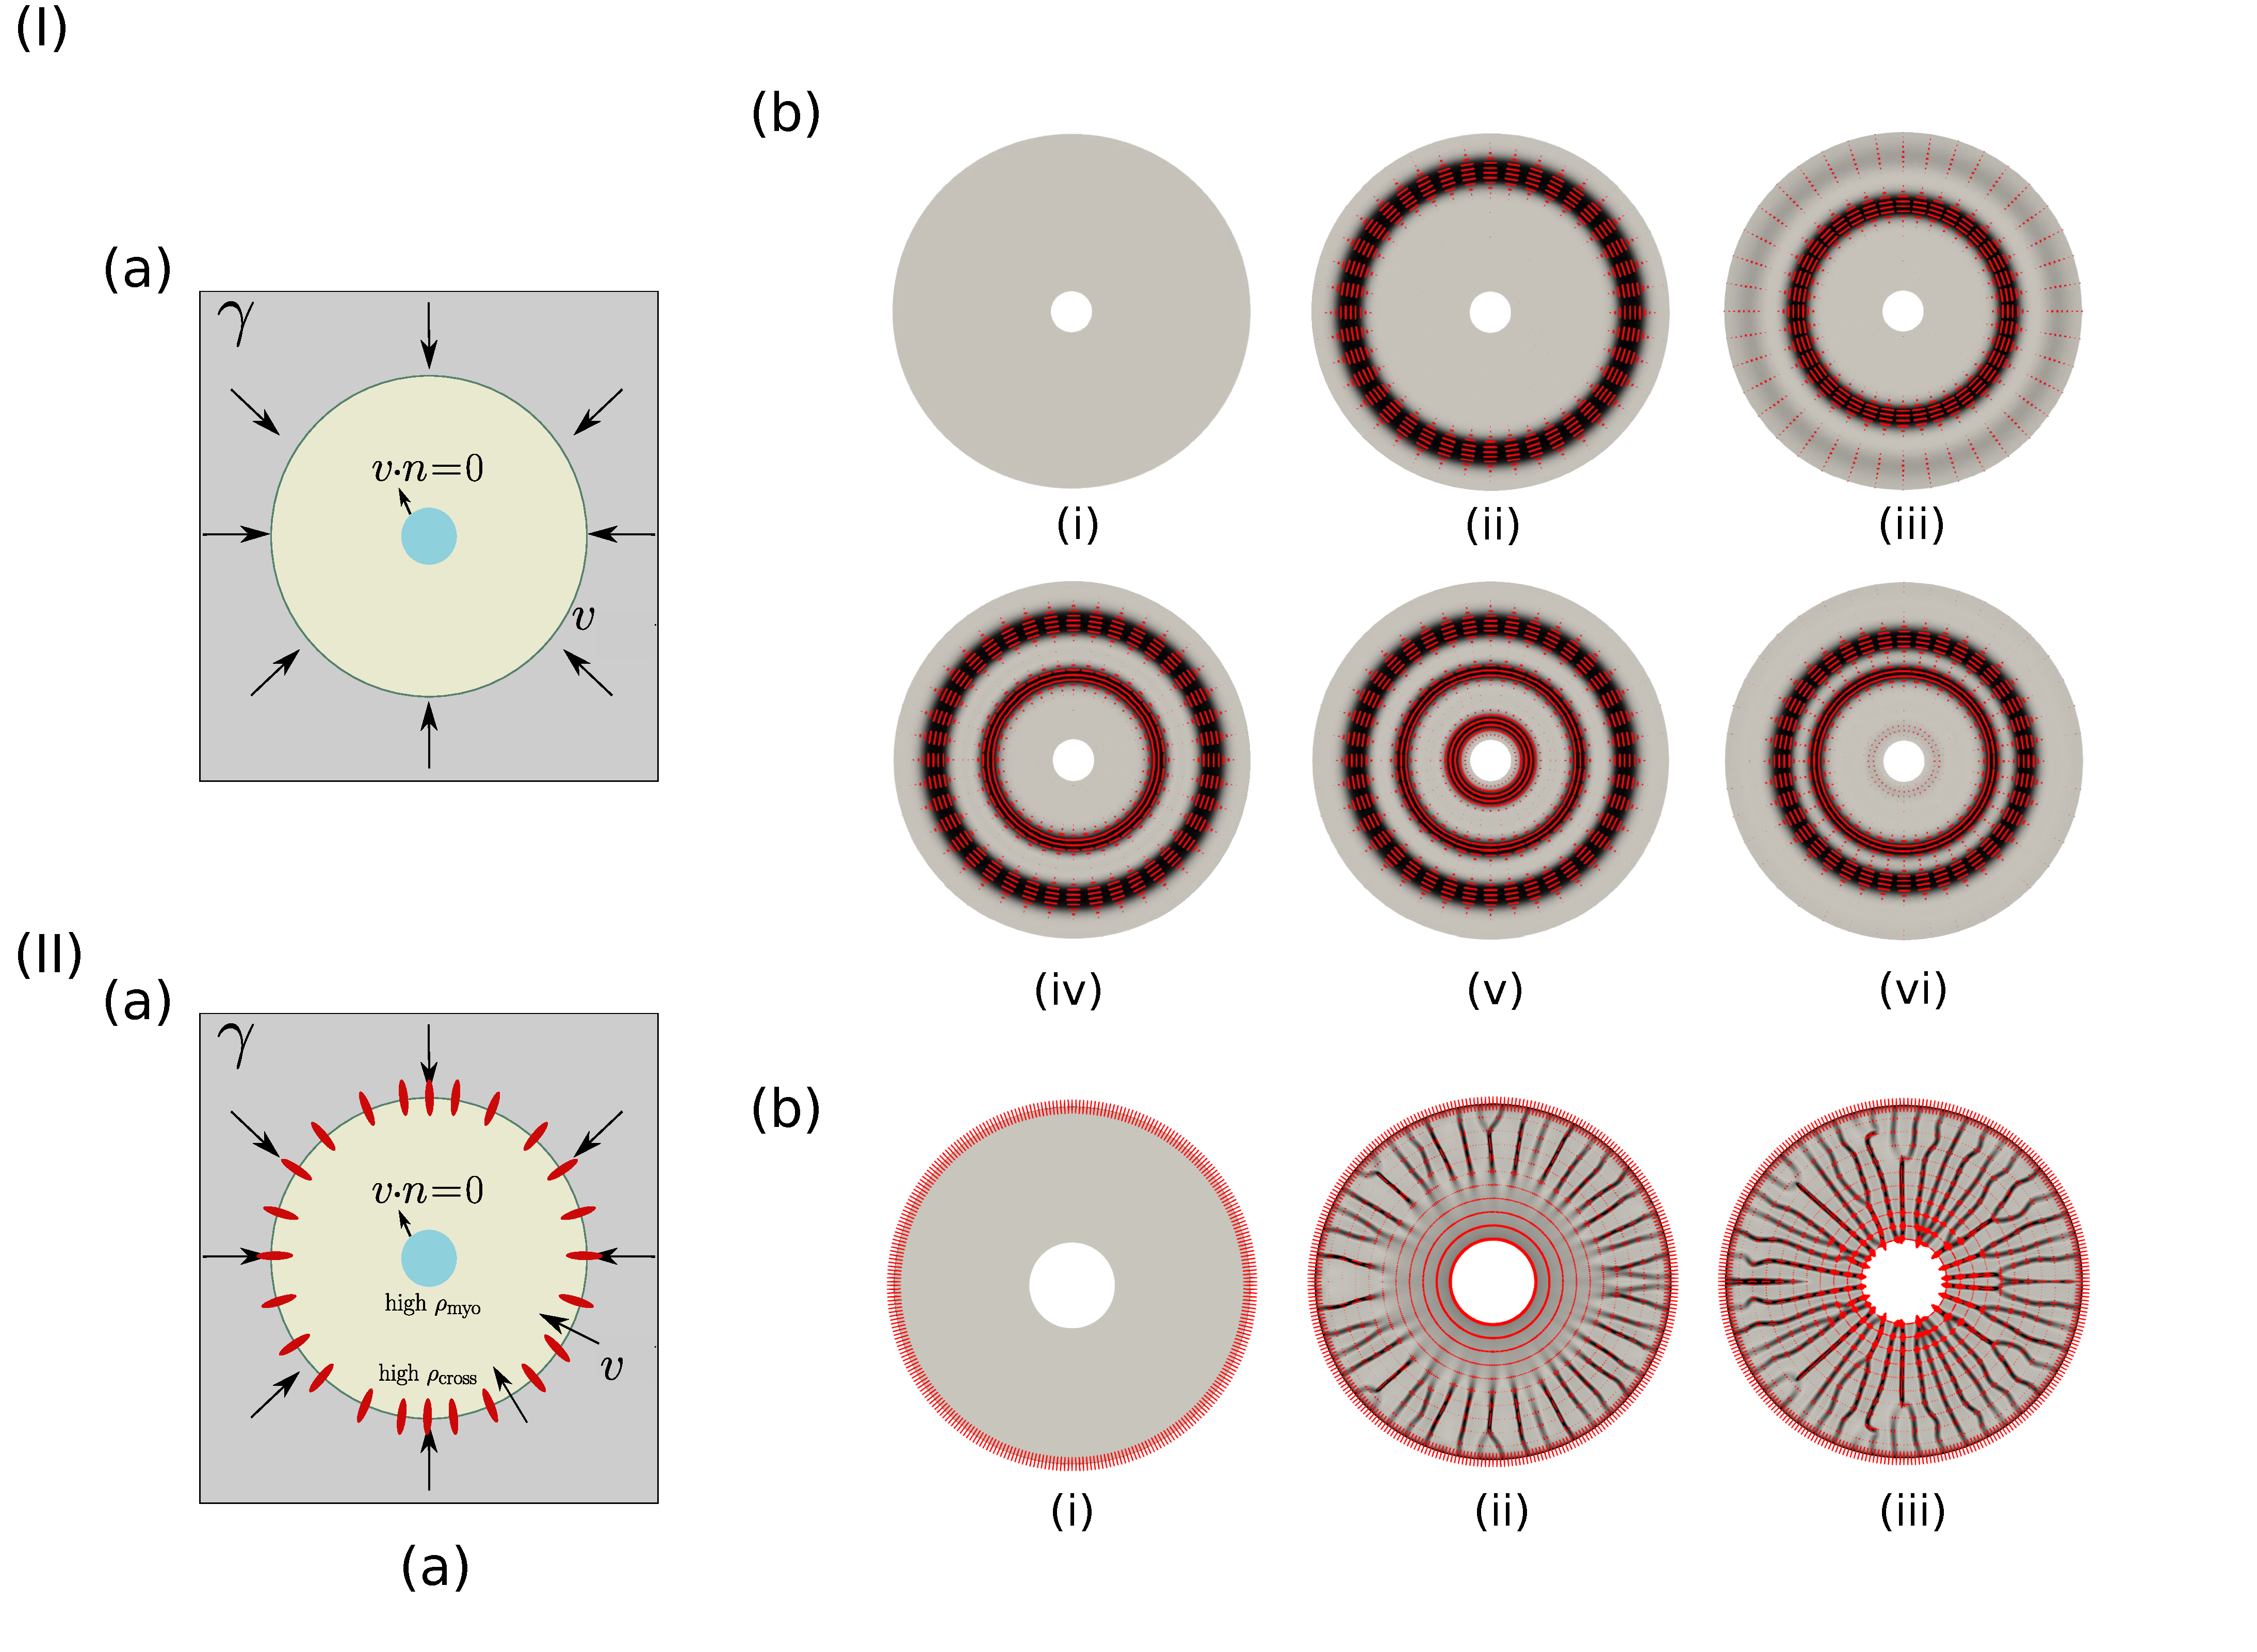
\includegraphics[width=1\textwidth]{chap_10_fig.pdf}
	\caption{\textbf{Self-organization of actin bundles in a cell-like geometry and boundary conditions}. (I.a) Domain and boundary conditions leading to the self-organization of transverse stress fibers. (I.b) Snapshots illustrating the development of a self-organized pulsating dynamical state in which transverse bundles nucleate near the cell periphery, move inwards, and disassemble near the nucleus. (II.a) Domain and boundary conditions leading to the self-organization of radial stress fibers. (II.b) Snapshots showing the self-organization radial nematic bundles from the leading edge and elongating to reach the nucleus.}
	\label{fig::1_chap10}
\end{figure}

Preliminary results with the extended model are illustrated in Fig.~\ref{fig::1_chap10} for different boundary conditions. We first considered a radial inwards flow in the outer boundary and zero normal flow at the inner boundary, modeling actin polymerization at the leading edge and the steric hinderance of the nucleus, Fig.~\ref{fig::1_chap10}(I). Starting from a uniform and isotropic gel, the system self-organizes transverse dense nematic bundles as follows: (I.b.i) The actin polymerized at the leading edge flows radially toward the center of the cell. As the actin network flows, the substrate exerts an opposing friction force proportional to the polymerization velocity. This impediment to the flow results in the densification of the gel at a distance similar to the hydrodynamic length $\ell_0$ from the leading edge. As the flow slows down due to friction, the actin network experience a local compression favoring network alignment tangential to the leading edge. (I.b.ii) The active alignment controlled by $\lambda_\odot$ and triggered by the incipient densification and ordering further increases alignment and condensation of the dense nematic arch. (I.b.iii-v) The arch being contractile, it moves inwards due to a Laplace-like force. As it moves inwards, a new arch is nucleated in the cell periphery by the same mechanism. (I.b.vi) As soon as an arch reaches the proximity of the nucleus, in agreement with observations of myosin-II depletion, we drop activity leading to arch disassembly. This sequence of events leads to a  pulsatile flow where a train of contractile arches self-organize close to the leading edge, flow radially, and disintegrate close to the cell nucleus,  \href{https://github.com/waleedmirzaPhD/movies_thesis.git}{Movie~9.1}.



Next, along with the velocity boundary conditions, we prescribed homeotropic boundary conditions for the nematic field consistent with the idea that, as the polar lamellipodium moves backward and loses polarity, it retains some nematic orientational order. Furthermore, we imposed and increased $\rho_{\rm cross}$ at the leading edge and an increased $\rho_{\rm myo}$ close to the nucleus \cite{tee2015, lehtimaki2021}, Fig.~\ref{fig::1_chap10}(II). As shown in the Fig.~\ref{fig::1_chap10} and in  \href{https://github.com/waleedmirzaPhD/movies_thesis.git}{Movie~9.2}, these conditions break the polar symmetry and lead to self-organized regularly spaced radial bundles with high nematic order and density at the leading edge. Once nucleated, they elongate as they are advected towards the nucleus due to the inwards polymerization velocity boundary condition.

These preliminary calculations suggest that the complex and dynamical stress fiber patterns in adherent may result from the modulation by cell geometry, heterogeneity, and boundary conditions of the intrinsic ability of the actin cytoskeleton to self-organize dense nematic bundles.

\subsection*{Systematic understanding of the interplay between shape and self-organized nematic structures}

Chapter~\ref{chap_8} has illustrated the tight coupling between cortical flows, density accumulation, nematic ordering and cell shape during cell morphogenesis. Towards a comprehensive mapping between active gel parameters and distinct self-organized dynamical modes involving dense nematic structures, we plan to perform linear stability analysis of the proposed active nematic gel on a deformable surface. Such a study, along with  nonlinear simulations avoiding the assumption of axisymmetry, may elucidate the conditions leading to cellular oscillations \cite{gorfinkiel2016,maitre2015}, to robust division \cite{yoshizaki2003}, to incomplete furrowing and cell elongation \cite{Dong}, or to polarized motility modes \cite{Ruprecht:2015aa}.
 
Likewise, on liquid crystal active nematic surfaces, defects are known to generate out-of-plane forces and hence trigger shape changes. This mechanism serves as a precursor of morphogenesis. For instance, during Hydra development, the locations of the early  mouth, foot, and tentacles correlate with $+1$ vortex-like defects \cite{maroudas2021}. Similar defect-induced shape transformations have been observed in active nematic vesicles \cite{keber2014} or in  myoblast cell cultures \cite{guillamat2020}. These and other defect-driven active morphogenetic events can be understood with the theoretical and computational models proposed in Chapters \ref{chap_7} and \ref{chap_9}.

